\actTitle{3.3 - Logarithmic Functions}

\videoLink{Section 3.3}{https://www.youtube.com/playlist?list=PLYHZK3b8UFw0UKAko9PhlIZXI78LYusTN}

\noindent \textbf{Topics:}  exponential functions, compound interest, the number $e$, exponential functions with base $e$, growth and decay\\

\noindent \textbf{Student Learning Outcomes:}
\begin{enumerate}
\item Students will be able to recognize a logarithic function graphically and algebraically.
\item Students will be able to evaluate the logarithmic expressions.
\item Students will be able to apply basic logarithmic properties.
\end{enumerate}

\hrule 

\bigskip

\subsection{Logarithmic Functions} ~

\noindent\begin{tabular}{ | l  |} \hline
\noindent  Let $a$ be a positive real number different from 1. The \emph{logarithm of $x$ with base $a$} is defined by   \\
\hspace{1.5in} $y = \log_a(x)$    if and only if   $a^y=x$. \\  \hline
\end{tabular} \\

\noindent Above, the left-hand equation is said to be in
\emph{logarithmic form}, while the right-hand equation is said to be
in \emph{exponential form}. The equations are \emph{equivalent}: they
have the same solutions.

\noindent
\begin{tabular}{m{0.4\textwidth}@{\hspace{2em}}m{0.5\textwidth}}
  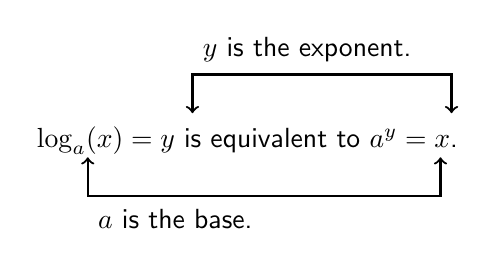
\begin{tikzpicture}[y=0.7cm, x=0.7cm,font=\sffamily]
    \node[anchor=west] at (0,0) {$\log_a(x)=y$ is equivalent to $a^y=x$.};
    \draw[thick,<->] (1.1,-0.3) -- (1.1,-1) 
       node[anchor=north west,yshift=-1,pos=1] {$a$ is the base.}
       -- (7.5,-1) -- (7.5,-0.3);
    \draw[thick,<->] (3,0.5) -- (3,1.2)
       node[anchor=south west,yshift=1,pos=1] {$y$ is the exponent.}
       -- (7.7,1.2) -- (7.7,0.5);
     \end{tikzpicture}
  &
  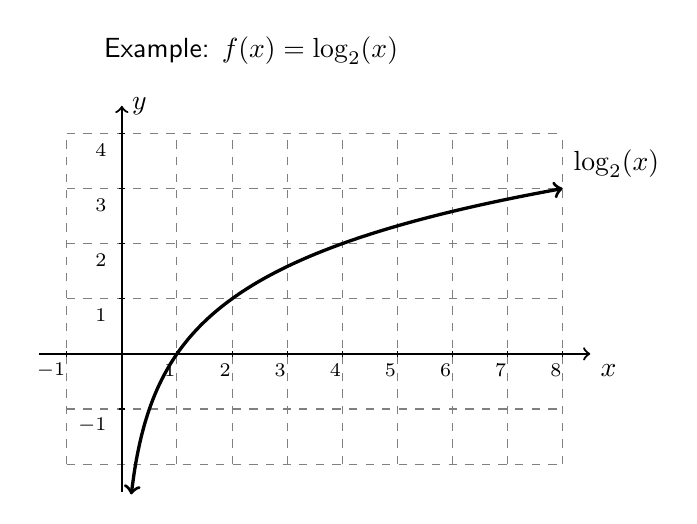
\begin{tikzpicture}[y=0.7cm, x=0.7cm,font=\sffamily]
    \begin{scope}
      %% ticks
      \draw[step = 1.0, gray,dashed] (-1,-2) grid (8,4);
      %% axis
      \draw[thick,->] (-1.5,0) -- coordinate (x axis mid) (8.5,0)
          node[anchor = north west] {$x$};
      \draw[thick,->] (0,-2.5) -- coordinate (y axis mid) (0,4.5) node[anchor=west] {$y$};

      \foreach \y in {-1,1,2,3,4} {
        \draw (1pt, \y) -- (-1pt, \y)
            node[font=\scriptsize,yshift=-6,xshift=-1,anchor=east] {$\y$};
      }
      \foreach \x in {-1,1,2,3,4,5,6,7,8} {
        \draw (\x,1pt) -- (\x,-1pt) node[font=\scriptsize,yshift=-5,xshift=3,anchor=east] {$\x$};
      }

      \node[anchor=west,align=left] at (-0.5,5.5) {Example: $f(x)=\log_2(x)$};
      
      \begin{scope}
        %% \clip(-4,-1) rectangle (8,5);
        \draw[scale=1.0,domain=0.17:8,smooth,variable=\x,very thick,black,samples=100,<->]
            plot ({\x},{ln(\x)/ln(2)}) node[anchor=south west] {$\log_2(x)$};
      \end{scope}
     \end{scope}

  \end{tikzpicture}
\end{tabular}

\begin{enumerate}
\item Write in exponential form.  \\
model: $\log_a(x)=y$ \hspace{1in} $\log_2 (16) = 4$ \hspace{1in} $\log_p (13) = y$\\[1in]

\item Write in logarithmic form. \\
model: $a^y = x$  \hspace{1in} $4^{-3} = \dfrac{1}{64}$ \hspace{1in} $\pi^t = 9.4$ \\[.5in]


\item The expression $\log x$, called the \emph{common logarithm}, is shorthand for $\log_{10}(x)$. Write in logarithmic form: $10^{2x+3} = 7$. \\[.5in]


\item The expression $\log x$, called the \emph{common logarithm}, is shorthand for $\log_{10}(x)$. Write in logarithmic form: $10^{2x+3} = 7$. \\[.5in]

\item Find the domain of the function $f(x) = \ln (9-6x)$. \\[.8in]



\subsection{Evaluating Logarithmic Expressions}
  
\item Find the number, if possible. Rewrite in exponential form, either to solve, or to check.
$\log_2 \left(  \dfrac{1}{8} \right)$  \hspace{1in} $\log_3 (27)$  \hspace{1in} $\log_4(0)$   \hspace{1in} $\log_b\left(\dfrac{1}{b^3}\right)$ \\[1in]




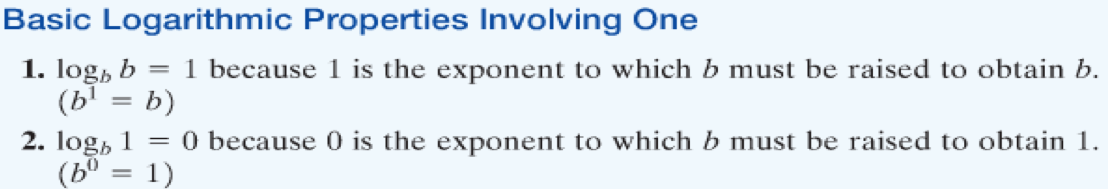
\includegraphics[scale=.9]{logprop1}
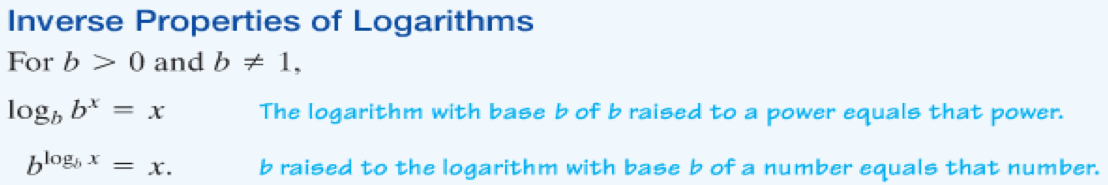
\includegraphics[scale=.9]{logprop2}

\item Evaluate the common and natural logarithms.\\
$\log (100,000)$  \hspace{1in} $\log (0.001)$  \hspace{1in} $\ln (e^4)$   \hspace{1in} $\ln \left(\dfrac{1}{e}\right)$ \\

\subsection{Graphing Logarithmic Functions} ~

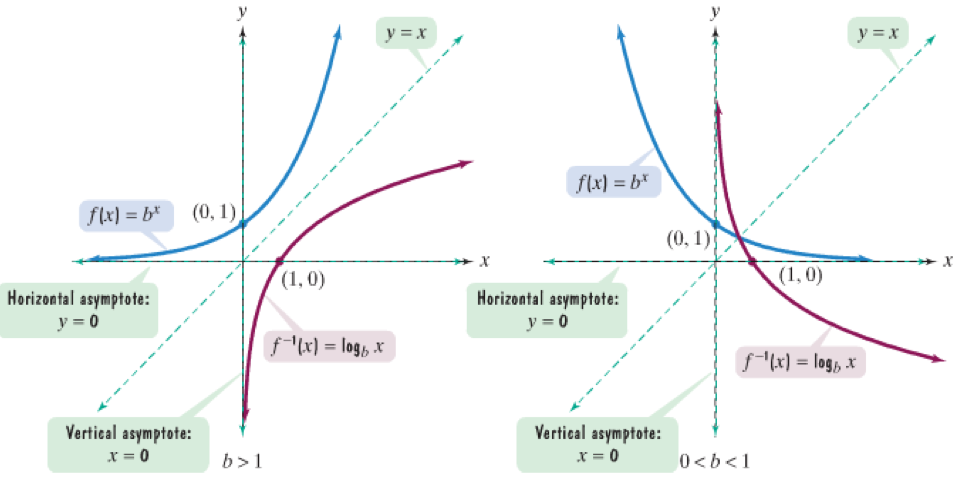
\includegraphics{loggraph}

\item Graph $\log_2 x$ and $\log_{1/4} x$\\
      \noindent
      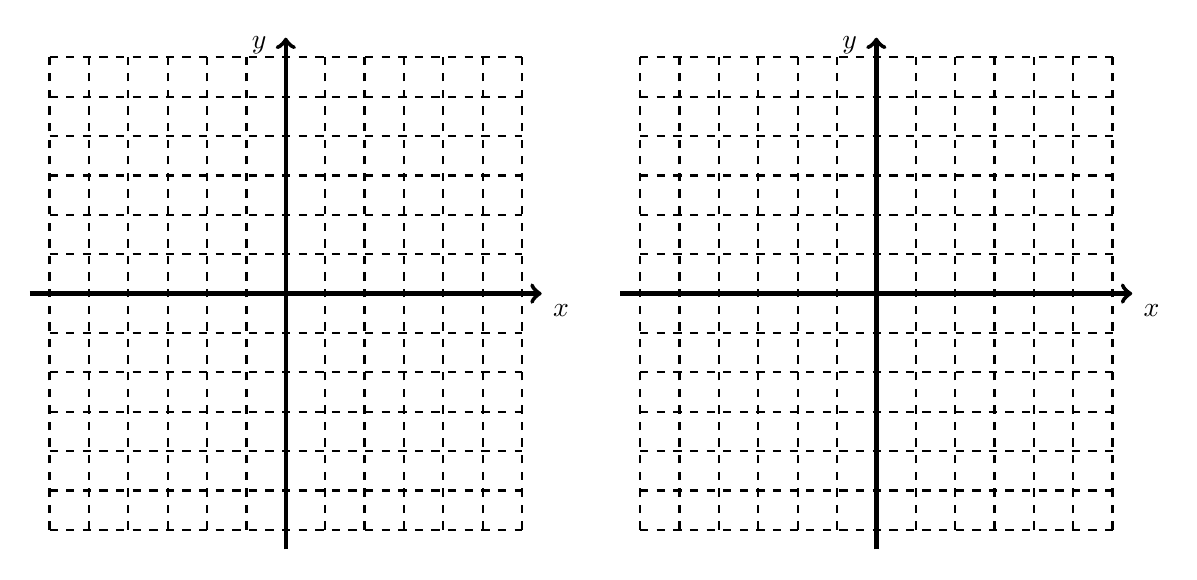
\begin{tikzpicture}[y=0.5cm, x=0.5cm,font=\sffamily]
        \begin{scope} %[shift={(0,8)}]
          %% ticks
          \draw[xstep = 1, ystep=1.0,black,dashed,thick] % very thin,opacity=0.85,
                 (-6.0,-6.0) grid ( 6.0, 6.0);
             %% axis
           \draw[ultra thick,->] (-6.5,0) -- coordinate (x axis mid) (6.5,0)
                node[anchor = north west] {$x$}; 
           \draw[ultra thick,->] (0,-6.5) -- coordinate (y axis mid) (0,6.5) 
                node[anchor = east,shift={(-0.2,-0.2)}]  {$y$};

           %\foreach \y in {-1,1,...,4} {
           %   \draw (1pt, \y) -- (-1pt, \y) node[yshift=-6,xshift=1,anchor=west] {$\y$};
           % }
           %\foreach \x in {-3,-2,-1,1,2,3} {
           %   \draw (\x,1pt) -- (\x,-1pt) node[yshift=-5,xshift=-1,anchor=east] {$\x$};
           % }

          \end{scope}

        \begin{scope} [shift={(15,0)}]
          %% ticks
          \draw[xstep = 1, ystep=1.0,black,dashed,thick] % very thin,opacity=0.85,
                 (-6.0,-6.0) grid ( 6.0, 6.0);
             %% axis
           \draw[ultra thick,->] (-6.5,0) -- coordinate (x axis mid) (6.5,0)
                node[anchor = north west] {$x$}; 
           \draw[ultra thick,->] (0,-6.5) -- coordinate (y axis mid) (0,6.5) 
                node[anchor = east,shift={(-0.2,-0.2)}]  {$y$};

           %\foreach \y in {-1,1,...,4} {
           %   \draw (1pt, \y) -- (-1pt, \y) node[yshift=-6,xshift=1,anchor=west] {$\y$};
           % }
           %\foreach \x in {-3,-2,-1,1,2,3} {
           %   \draw (\x,1pt) -- (\x,-1pt) node[yshift=-5,xshift=-1,anchor=east] {$\x$};
           % }

          \end{scope}

        \end{tikzpicture}


\end{enumerate}

\noindent \textbf{Student Learning Outcomes Check}

\begin{enumerate}
\item Can you recognize a logarithic function graphically and algebraically?
\item Can you evaluate the logarithmic expressions?
\item Are you able to apply basic logarithmic properties?

\end{enumerate}

\noindent \textbf{If any of your answers were no, please ask about these topics in class.}


